\documentclass[12pt]{article}
\usepackage{amsmath}
\usepackage{graphicx}
\usepackage{geometry}
\usepackage{booktabs}

\geometry{margin=1in}

\title{Lab 1: Euler Buckling of Columns}
\author{Jacob Vaught \\
        Mechanical Engineering Lab II}
\date{\today}

\begin{document}

\maketitle

\tableofcontents
\newpage

\section{Introduction}
\label{sec:introduction}

The objective of this lab is to demonstrate various buckling problems using Euler’s formula for columns with different boundary conditions. The experiment focuses on measuring the critical buckling load \( P_{\text{cr}} \) and using these measurements to calculate the modulus of elasticity \( E \) for the material. The four boundary conditions investigated are fixed-free, pinned-pinned, fixed-pinned, and fixed-fixed.

\section{Experimental Procedures}
\label{sec:procedures}

\subsection{Equipment Used}
\label{subsec:equipment}

The experiment utilized the WP 121 Demonstration Unit for Euler Buckling. This unit includes various components such as weights of different masses, which were used to apply the necessary loads to the metal strips acting as columns. Each strip was set up to correspond to a different boundary condition, or `case' of fixity, allowing for the observation of buckling behavior under different constraints. To facilitate clear visualization of the deformation, a white background wall was provided behind the columns.

\begin{figure}[h!]
\centering
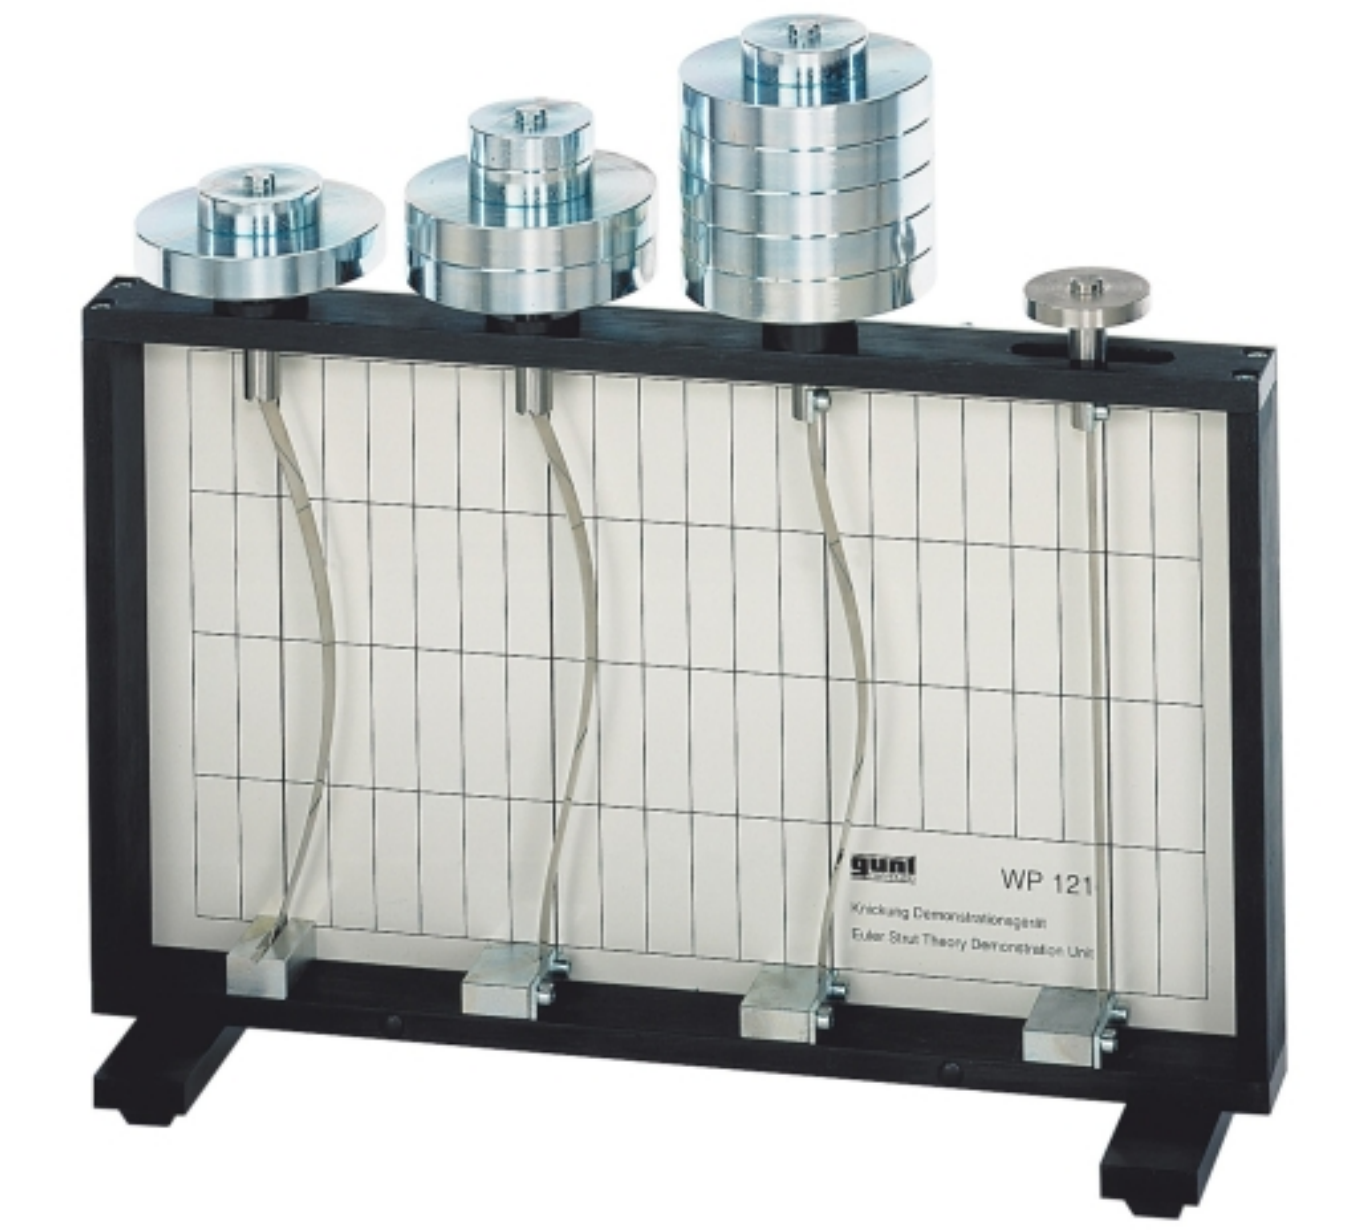
\includegraphics[width=0.8\textwidth]{Euler_Buckling.png}
\caption{WP 121 Demonstration Unit for Euler Buckling}
\label{fig:wp121}
\end{figure}



\subsection{Measurements Performed}
\label{subsec:measurements}

During the lab, several key measurements were performed to ensure accurate analysis. The height (\( h \)), width (\( b \)), and length (\( L \)) of each metal strip were measured using a caliper, allowing precise calculation of the moment of inertia \( I \). These measurements were repeated five times for each boundary condition—fixed-free, pinned-pinned, fixed-pinned, and fixed-fixed—enabling the calculation of average values and the potential for statistical analysis. The critical buckling load (\( F_{\text{crit}} \)) was also recorded five times for each case, providing reliable data for evaluating the buckling behavior. For all cases, the buckling mode was consistent and identified as mode 1. Additionally, the buckling pattern of each strip was observed and documented to support the analysis.


\subsection{Procedures}
\label{subsec:procedure}

First, the WP 121 Demonstration Unit was assembled, and the correct configuration for the desired boundary condition—whether fixed-free, pinned-pinned, fixed-pinned, or fixed-fixed—was ensured. Once the setup was complete, the precise dimensions of each metal strip, including height, width, and length, were measured using a caliper to guarantee accuracy in subsequent calculations.

Following the measurement of dimensions, a series of loads was applied to each metal strip to induce buckling. Weights of 1N and 5N were used incrementally, ensuring even application of the load. The load at which buckling occurred, denoted as the critical buckling load (\( F_{\text{crit}} \)), was carefully recorded. This process was repeated five times for each boundary condition to obtain a reliable average value and to facilitate statistical analysis.

\section{Discussion}
\label{sec:discussion}

\subsection{Sources of Uncertainty}
\label{subsec:uncertainty}

Several factors contributed to uncertainty in the results:

\begin{itemize}
    \item Small inaccuracies in measuring dimensions like length and width.
    \item Improper setup could lead to uneven load distribution.
    \item Variations in material properties like \( E \) or non-homogeneous material.
    \item Inconsistent application of weights during the experiment.
    \item Temperature and humidity variations affecting material behavior.
\end{itemize}

\subsection{Recommendations}
\label{subsec:recommendations}

To reduce uncertainty:

\begin{itemize}
    \item Enhance measurement accuracy with better instruments.
    \item Ensure consistent setup for each trial.
\end{itemize}


\subsection{Comparison with Literature Values}
\label{subsec:comparison}

The calculated modulus of elasticity \( E \) was compared with standard literature values for the material used. According to the user manual, the relevant properties for the steel strips are as follows:
\begin{itemize}
    \item Bar length: 180 mm
    \item Bar cross-section: 0.5 mm x 12 mm
    \item Material: Steel 1.4310, cold-worked
    \item Buckling loads: Approximately 2–32 N
    \item The modulus of elasticity \( E \) is approximately 200 GPa.
\end{itemize}

Any discrepancies between the experimental and literature values are analyzed in the context of the identified sources of uncertainty.


\section{Experimental Results and Analysis}
\label{sec:results}

\subsection{Measured Data}
\label{subsec:data}

\begin{table}[h!]
\centering
\caption{Values of \( K \) and \( n \) for Different Boundary Conditions}
\begin{tabular}{|c|c|c|}
\hline
\textbf{Boundary Condition} & \textbf{K (Effective Length Factor)} & \textbf{n (Buckling Mode)} \\ \hline
Fixed-Free    & 2.0  & 1 \\ \hline
Pinned-Pinned & 1.0  & 1 \\ \hline
Fixed-Pinned  & \(\sqrt{2}/2 \approx 0.707\)  & 1 \\ \hline
Fixed-Fixed   & 0.5  & 1 \\ \hline
\end{tabular}
\label{tab:K_n_values}
\end{table}

The modulus of elasticity \( E \) is derived from the critical buckling load \( P_{\text{cr}} \) and the moment of inertia \( I \) using Euler’s buckling formula:

\[
E = \frac{P_{\text{cr}} \cdot (K L)^2}{n^2 \pi^2 I}
\]

\[
I = \frac{h \cdot b^3}{12}
\]

\begin{table}[h!]
\centering
\caption{Fixed-Free Case Measurements}
\begin{tabular}{@{}lccccccc@{}}
\toprule
\textbf{Measurement} & \textbf{Trial 1} & \textbf{Trial 2} & \textbf{Trial 3} & \textbf{Trial 4} & \textbf{Trial 5} & \textbf{Average} & \textbf{Std Dev} \\ \midrule
\textbf{L (mm)} & 181 & 180 & 181 & 179 & 180 & 180.2 & 0.83666 \\
\textbf{h (mm)} & 11.9 & 12 & 11.8 & 11.9 & 12.1 & 11.94 & 0.114018 \\
\textbf{b (mm)} & 0.4 & 0.6 & 0.4 & 0.6 & 0.5 & 0.5 & 0.1 \\
\textbf{I\(_y\) (mm\(^4\))} & 0.063467 & 0.216 & 0.062933 & 0.2142 & 0.126042 & 0.124375 & 0.076179 \\
\textbf{P\(_{crit}\) (N)} & 4 & 5 & 5 & 4 & 5.3924 & 4.67848 & 0.639746 \\
\textbf{E (GPa)} & 836.8193 & 303.9636 & 1054.889 & 242.4973 & 561.789 & 495.0414 & 346.3788 \\
\bottomrule
\end{tabular}
\label{tab:fixed_free}
\end{table}

\begin{table}[h!]
\centering
\caption{Pinned-Pinned Case Measurements}
\begin{tabular}{@{}lccccccc@{}}
\toprule
\textbf{Measurement} & \textbf{Trial 1} & \textbf{Trial 2} & \textbf{Trial 3} & \textbf{Trial 4} & \textbf{Trial 5} & \textbf{Average} & \textbf{Std Dev} \\ \midrule
\textbf{L (mm)} & 181 & 180 & 181 & 179 & 180 & 180.2 & 0.83666 \\
\textbf{h (mm)} & 11.9 & 12 & 11.8 & 11.9 & 12.1 & 11.94 & 0.114018 \\
\textbf{b (mm)} & 0.4 & 0.6 & 0.4 & 0.6 & 0.5 & 0.5 & 0.1 \\
\textbf{I\(_y\) (mm\(^4\))} & 0.063467 & 0.216 & 0.062933 & 0.2142 & 0.126042 & 0.124375 & 0.076179 \\
\textbf{P\(_{crit}\) (N)} & 7 & 7 & 7 & 7 & 7 & 7 & 0 \\
\textbf{E (GPa)} & 366.1085 & 106.3872 & 369.2111 & 106.0926 & 182.3178 & 185.1718 & 132.9783 \\
\bottomrule
\end{tabular}
\label{tab:pinned_pinned}
\end{table}

\begin{table}[h!]
\centering
\caption{Fixed-Pinned Case Measurements}
\begin{tabular}{@{}lccccccc@{}}
\toprule
\textbf{Measurement} & \textbf{Trial 1} & \textbf{Trial 2} & \textbf{Trial 3} & \textbf{Trial 4} & \textbf{Trial 5} & \textbf{Average} & \textbf{Std Dev} \\ \midrule
\textbf{L (mm)} & 181 & 180 & 181 & 179 & 180 & 180.2 & 0.83666 \\
\textbf{h (mm)} & 11.9 & 12 & 11.8 & 11.9 & 12.1 & 11.94 & 0.114018 \\
\textbf{b (mm)} & 0.4 & 0.6 & 0.4 & 0.6 & 0.5 & 0.5 & 0.1 \\
\textbf{I\(_y\) (mm\(^4\))} & 0.063467 & 0.216 & 0.062933 & 0.2142 & 0.126042 & 0.124375 & 0.076179 \\
\textbf{P\(_{crit}\) (N)} & 16 & 14 & 15 & 16 & 15 & 15.2 & 0.83666 \\
\textbf{E (GPa)} & 418.4097 & 106.3872 & 395.5833 & 121.2486 & 195.3405 & 201.0436 & 149.7594 \\
\bottomrule
\end{tabular}
\label{tab:fixed_pinned}
\end{table}

\begin{table}[h!]
\centering
\caption{Fixed-Fixed Case Measurements}
\begin{tabular}{@{}lccccccc@{}}
\toprule
\textbf{Measurement} & \textbf{Trial 1} & \textbf{Trial 2} & \textbf{Trial 3} & \textbf{Trial 4} & \textbf{Trial 5} & \textbf{Average} & \textbf{Std Dev} \\ \midrule
\textbf{L (mm)} & 181 & 180 & 181 & 179 & 180 & 180.2 & 0.83666 \\
\textbf{h (mm)} & 11.9 & 12 & 11.8 & 11.9 & 12.1 & 11.94 & 0.114018 \\
\textbf{b (mm)} & 0.4 & 0.6 & 0.4 & 0.6 & 0.5 & 0.5 & 0.1 \\
\textbf{I\(_y\) (mm\(^4\))} & 0.063467 & 0.216 & 0.062933 & 0.2142 & 0.126042 & 0.124375 & 0.076179 \\
\textbf{P\(_{crit}\) (N)} & 32 & 33 & 33 & 32 & 31 & 32.2 & 0.83666 \\
\textbf{E (GPa)} & 418.4097 & 125.385 & 435.1416 & 121.2486 & 201.8519 & 212.9475 & 155.3397 \\
\bottomrule
\end{tabular}
\label{tab:fixed_fixed}
\end{table}

\newpage
\subsection{Error Propagation to Modulus of Elasticity}
\label{subsec:error_propagation}

The modulus of elasticity \( E \) is derived from the critical buckling load \( P_{\text{cr}} \) and the moment of inertia \( I \) using Euler’s buckling formula:

\[
E = \frac{P_{\text{cr}} \cdot (K L)^2}{n^2 \pi^2 I}
\]

\subsubsection{Error from \( P_{\text{cr}} \)}
\label{subsubsec:error_Pcrit}

Since \( E \) is directly proportional to \( P_{\text{cr}} \), any error \( \Delta P_{\text{cr}} \) in measuring the critical load directly affects \( E \):

\[
\frac{\Delta E}{E} = \frac{\Delta P_{\text{cr}}}{P_{\text{cr}}}
\]

\subsubsection{Error from Moment of Inertia \( I \)}
\label{subsubsec:error_I}

Given that \( E \) is inversely proportional to \( I \), the relative error in \( E \) is:

\[
\frac{\Delta E}{E} = -\frac{\Delta I}{I}
\]

\subsubsection{Combined Error Propagation}
\label{subsubsec:combined_error}

The overall error in \( E \) from both \( P_{\text{cr}} \) and \( I \) is calculated using the method of propagation of uncertainties, which combines independent errors in quadrature. The combined relative error is given by:

\[
\frac{\Delta E}{E} = \sqrt{\left(\frac{\Delta P_{\text{cr}}}{P_{\text{cr}}}\right)^2 + \left(\frac{\Delta I}{I}\right)^2}
\]

This approach, known as the root-sum-square (RSS) method, assumes that the errors in \( P_{\text{cr}} \) and \( I \) are independent and random, providing an estimate of the uncertainty in \( E \).

\subsection{Reported Results with 75\% Confidence}
\label{subsec:reported_results}


\subsubsection{Fixed-Free Case}
The modulus of elasticity for the Fixed-Free case is calculated as:

\[
\bar{E}_{\text{Fixed-Free}} = 495.0414 \text{ GPa}
\]

The standard deviation is:

\[
s_{E, \text{Fixed-Free}} = 346.3788 \text{ GPa}
\]

The 75\% confidence interval is:

\[
\text{CI}_{\text{Fixed-Free}} = 495.0414 \pm 171.325 \text{ GPa}
\]

This gives an interval of \( [323.716, 666.367] \) GPa. Since the real modulus of elasticity for the material is 200 GPa, this result is significantly higher and suggests that the test was not accurate for this boundary condition. The high standard deviation also indicates substantial variability in the measurements.

\subsubsection{Pinned-Pinned Case}
The modulus of elasticity for the Pinned-Pinned case is calculated as:

\[
\bar{E}_{\text{Pinned-Pinned}} = 185.1718 \text{ GPa}
\]

The standard deviation is:

\[
s_{E, \text{Pinned-Pinned}} = 132.9783 \text{ GPa}
\]

The 75\% confidence interval is:

\[
\text{CI}_{\text{Pinned-Pinned}} = 185.1718 \pm 65.773 \text{ GPa}
\]

This gives an interval of \( [119.398, 250.945] \) GPa. The real value of 200 GPa falls within this interval, indicating that the test for this boundary condition was relatively accurate, though the variability is still considerable.

\subsubsection{Fixed-Pinned Case}
The modulus of elasticity for the Fixed-Pinned case is calculated as:

\[
\bar{E}_{\text{Fixed-Pinned}} = 201.0436 \text{ GPa}
\]

The standard deviation is:

\[
s_{E, \text{Fixed-Pinned}} = 149.7594 \text{ GPa}
\]

The 75\% confidence interval is:

\[
\text{CI}_{\text{Fixed-Pinned}} = 201.0436 \pm 74.074 \text{ GPa}
\]

This gives an interval of \( [126.970, 275.117] \) GPa. The real modulus of 200 GPa is within this interval, suggesting that the test was fairly accurate, although the high standard deviation shows a significant spread in the results.

\subsubsection{Fixed-Fixed Case}
The modulus of elasticity for the Fixed-Fixed case is calculated as:

\[
\bar{E}_{\text{Fixed-Fixed}} = 212.9475 \text{ GPa}
\]

The standard deviation is:

\[
s_{E, \text{Fixed-Fixed}} = 155.3397 \text{ GPa}
\]

The 75\% confidence interval is:

\[
\text{CI}_{\text{Fixed-Fixed}} = 212.9475 \pm 76.834 \text{ GPa}
\]

This gives an interval of \( [136.114, 289.781] \) GPa. The real modulus of elasticity (200 GPa) is within this range, indicating that the test for this boundary condition was relatively accurate, but again, the high standard deviation suggests a broad spread in the data.

\end{document}
